\documentclass{article}\usepackage[]{graphicx}\usepackage[]{color}
% maxwidth is the original width if it is less than linewidth
% otherwise use linewidth (to make sure the graphics do not exceed the margin)
\makeatletter
\def\maxwidth{ %
  \ifdim\Gin@nat@width>\linewidth
    \linewidth
  \else
    \Gin@nat@width
  \fi
}
\makeatother

\definecolor{fgcolor}{rgb}{0.345, 0.345, 0.345}
\newcommand{\hlnum}[1]{\textcolor[rgb]{0.686,0.059,0.569}{#1}}%
\newcommand{\hlstr}[1]{\textcolor[rgb]{0.192,0.494,0.8}{#1}}%
\newcommand{\hlcom}[1]{\textcolor[rgb]{0.678,0.584,0.686}{\textit{#1}}}%
\newcommand{\hlopt}[1]{\textcolor[rgb]{0,0,0}{#1}}%
\newcommand{\hlstd}[1]{\textcolor[rgb]{0.345,0.345,0.345}{#1}}%
\newcommand{\hlkwa}[1]{\textcolor[rgb]{0.161,0.373,0.58}{\textbf{#1}}}%
\newcommand{\hlkwb}[1]{\textcolor[rgb]{0.69,0.353,0.396}{#1}}%
\newcommand{\hlkwc}[1]{\textcolor[rgb]{0.333,0.667,0.333}{#1}}%
\newcommand{\hlkwd}[1]{\textcolor[rgb]{0.737,0.353,0.396}{\textbf{#1}}}%
\let\hlipl\hlkwb

\usepackage{framed}
\makeatletter
\newenvironment{kframe}{%
 \def\at@end@of@kframe{}%
 \ifinner\ifhmode%
  \def\at@end@of@kframe{\end{minipage}}%
  \begin{minipage}{\columnwidth}%
 \fi\fi%
 \def\FrameCommand##1{\hskip\@totalleftmargin \hskip-\fboxsep
 \colorbox{shadecolor}{##1}\hskip-\fboxsep
     % There is no \\@totalrightmargin, so:
     \hskip-\linewidth \hskip-\@totalleftmargin \hskip\columnwidth}%
 \MakeFramed {\advance\hsize-\width
   \@totalleftmargin\z@ \linewidth\hsize
   \@setminipage}}%
 {\par\unskip\endMakeFramed%
 \at@end@of@kframe}
\makeatother

\definecolor{shadecolor}{rgb}{.97, .97, .97}
\definecolor{messagecolor}{rgb}{0, 0, 0}
\definecolor{warningcolor}{rgb}{1, 0, 1}
\definecolor{errorcolor}{rgb}{1, 0, 0}
\newenvironment{knitrout}{}{} % an empty environment to be redefined in TeX

\usepackage{alltt}
\usepackage{graphicx}
\usepackage{rotating}
\usepackage{graphics}
\usepackage{latexsym}
\usepackage{color}
\usepackage{listings} % allows for importing code scripts into the tex file
\usepackage{wrapfig} % allows wrapping text around a figure
\usepackage{lipsum} % provides Latin text to fill up a page in this illustration (do not need it otherwise!)

% Approximately 1 inch borders all around
\setlength\topmargin{-.56in}
\setlength\evensidemargin{0in}
\setlength\oddsidemargin{0in}
\setlength\textwidth{6.49in}
\setlength\textheight{8.6in}

% Options for code listing; from Patrick DeJesus, October 2016
\definecolor{codegreen}{rgb}{0,0.6,0}
\definecolor{codegray}{rgb}{0.5,0.5,0.5}
\definecolor{codepurple}{rgb}{0.58,0,0.82}
\definecolor{backcolour}{rgb}{0.95,0.95,0.92}
\lstdefinestyle{mystyle}{
	backgroundcolor=\color{backcolour},   commentstyle=\color{codegreen},
	keywordstyle=\color{magenta},
	numberstyle=\tiny\color{codegray},
	stringstyle=\color{codepurple},
	basicstyle=\footnotesize,
	breakatwhitespace=false,         
	breaklines=true,                 
	captionpos=b,                    
	keepspaces=true,                 
	numbers=left,                    
	numbersep=5pt,                  
	showspaces=false,                
	showstringspaces=false,
	showtabs=false,                  
	tabsize=2
}

%"mystyle" code listing set
\lstset{style=mystyle}
%\lstset{inputpath=appendix/}


\title{Predictions Survival Rates based on Vitals 
taken at Admission and Discharge/Death} 
\author{}
\IfFileExists{upquote.sty}{\usepackage{upquote}}{}
\begin{document} 

\maketitle
\begin{center}
\Large{Abstract}
\end{center}
\qquad Shock is a serious life condition which can lead to death in a person. In Southern California, data was collected on patients twice when they were initially admitted and final vitals. Significant contributors to a patient's survival rate was their Shock Type, Mean Arterial Pressure, Mean Central Venous Pressure, Body Surface Index, Urinary Output, and Red Cell Index. Shock Type was a significant indicator on whether the patient will survive. Interaction terms were considered in the model selection, but ultimately not used due to stepAIC. Take a patient with Other Shock, MAP of 70, MCVP of 100, BSI of 150, UO of 75, RCI of 150. This patient has 17676.65 odds more likely to die.
\section{Introduction}
\qquad Death by shock is a life threatening condition where the body does not get enough blood flow. There was data collected in Southern California on patients when they were being admitted and final measurements. There were 43 patients who succumbed to their conditions and 69 who survived. Specifically, 40 of the deaths were due to some category of shock. Only 3 deaths were not of shock. This analysis will determine what the best indicators are to predict the patient's survival rate based on measurements taken when the patient got admitted and final vitals measured. Logistic Regression will be applied because the response is binary. There is a hypothesis that shock type will greatly affect whether a patient survives.

%survival by sex
\begin{table}[ht]
\centering
\caption{Survival by Sex Table}
\label{sex}
\begin{tabular}{rrr}
  \hline
 & Died & Survived \\ 
  \hline
Female &  26 &  28 \\ 
  Male &  17 &  41 \\ 
   \hline
\end{tabular}
\end{table}


\section{Methods}
\qquad There were 112 critically ill patients that were admitted to an Emergency room. Vitals were taken upon admission and taken again right before death or discharge. Record showed whether the vitals were taken upon admission or as final measurements. ID was the patient's identification. Age was the age of the patient in years. Sex of the patient was either male (1) or female (2). Height is the height of the patient in cm's. Survive was whether the patient had survived (0) or died (1). Shock type was the patient's status and what kind of shock they were in: Non-Shock meant the patient did not have any shock. Hypovolemic Shock is losing severe amount of blood. Cardiogenic Shock is when a patient's heart cannot pump enough blood to meet the body's demand. Bacterial Shock is a complication of certain bacterial infections. Neurogenic Shock is irregular blood circulation usually leading to low blood pressure often caused by trauma or injury to the spinal cord. SBP was their systolic blood pressure measured in mmHg. MAP was the patient's mean arterial pressure measured in mmHg. HR was the patient's heart rate in beats/mins. DBP is diastolic blood pressure measured in mmHg. MCVP is mean central venous water pressure measured in cm. BSI is the patient's body surface index measured in $m^2$. CI is cardiac index measured in liters/(min * $m^2$). AT is appearance time of physical symptoms in seconds. MCT is mean circulation time measured in seconds. UO is urinary output is measured mL/hr. PVI is Plasma volume index is measured in mL/kg. RCI is the red cell index measured in mL/kg. HG is hemoglobin is gm/100mL. HCT is hematocrit is measured in percent. Record is whether the initial or final measurement was taken. The analysis will be conducted using R/RStudio. 


%survival by shock type
\begin{table}[ht]
\centering
\caption{Survival by Shock Type Table}
\label{shock}
\begin{tabular}{rrrrrrr}
  \hline
 & Bacterial & Cardiogenic & Hypovolemic & Neurogenic & Non-Shock & Other \\ 
  \hline
  Survived &   9 &  10 &   7 &   9 &  31 &   3 \\ 
  Died &   6 &  10 &  10 &   7 &   3 &   7 \\ 
   \hline
\end{tabular}
\end{table}

\section{Results}
\subsection{Exploratory Data Analysis}
\qquad In table \ref{sex}, there was a surprising discovery that men survived at a rate more than double compared to women. In table \ref{shock} showed that the largest group that survived was those who were not in shock. In these tables showed that males with a non-shock condition will likely survive. By using the function stepAIC on all possible models, the model with the least of amount of penalties still had non significant terms. Manually, the terms that were not significant by p-values were dropped one-by-one out of the model, but dropped too many covariates including shock type. Eventually, the model contained six predictor variables that were not highly correlated with each other shown in figure 2 in the appendix. The correlation plot of all variables showed that the variables SBP, DBP, and MAP were highly correlated. MCT was highly correlated to AT. HCT was highly correlated to HG. MCT and AT were inversely correlated to CI. With dimension reduction and model selection, the model was lowered to 6 covariates. All variables except for survive, sex, shock type, and record were continuous.
\subsection{Model Fitting/Inferences}
\qquad 

\begin{figure}
\centering
\label{diagnostics}
\caption{Diagnostic Plot of the Final Model}
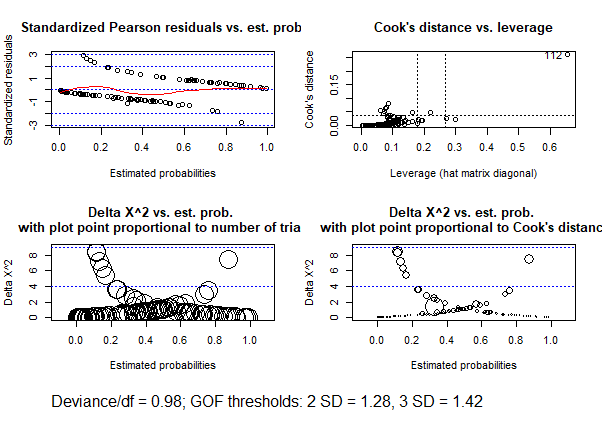
\includegraphics{diagnostics.png}
\end{figure}


\qquad Interpreting an odds ratio is is not too difficult. Any odds ratio at 1 does not in
influence the response. Odds ratios that are between 0 and 1 are (1 - odds ratio) * 100\% less odds of  dying. But with an odds ratio greater than 1 and less than 2, then the patient has (odds ratio - 1)
* 100\% more odds of dying.
Patients that had Cardiogenic Shock had 2.53 more likely odds in dying. Patients with Hypovolemic Shock had 3.52 more likely odds in dying. Patients with Neurogenic Shock had 2.28 more likely odds in dying. Patients with no shock had 64\% decrease in odds of dying. Patients with other shock types had 12.21 more likely odds of dying. Patients with every 1 unit MAP increase, decreases their odds of dying by 3\%. Patients with every 1 unit MCVP increase, increases their odds of dying by 1\%. Patients with every one unit increase of BSI, their odds of dying decrease by 3\%. Patients with every 1 unit of UO increases decreases their odds of dying by 1\%. Every increase of RCI in a patient, decreases their odds of dying by 1\%.
With this model, a patient's odds of death can be determined. Based on table \ref{odds}, take a patient with Other Shock, MAP of 70, MCVP of 100, BSI of 150, UO of 75, RCI of 150. This patient has 17676.65 odds more likely to die.
 
\qquad In the diagnostic plots figure 1 showed an influential point of patient 112. Looking at the Delta $X^2$ plot showed no significant impact to the model since all probabilities were contained under the $2^{nd}$ dotted line. Applying the Homser-Lemeshow test with 3 bins, the p-value is 0.13 means fail to reject the chosen model. The other thing of note is the pattern in the plot of the Standardized Pearson residuals vs estimated probabilities which seems to have 2 parallel lines. This is due to the limited number of observations and the data set itself. The confusion matrix table \ref{confuse} had a sensitivity of 71\% and a specificity of 74\%. It would be ideal to have both metrics above 90\% or at least optimally above 80\%.



\begin{table}[ht]
\centering
\caption{Odds Ratios with 95\% CI Odds Ratios}
\label{odds}
\begin{tabular}{ccccc}
  \hline
 &Coefficients&Odds Ratio & 2.5 \% & 97.5 \% \\ 
  \hline
(Intercept)&6.14& 462.70 & 3.75 & 99681.27 \\ 
  Cardiogenic Shock&0.93& 2.54 & 0.52 & 13.59 \\ 
  Hypovolemic Shock&1.26&3.52 & 0.63 & 22.36 \\ 
  Neurogenic Shock&0.82&2.28 & 0.42 & 13.44 \\ 
  Non-Shock&-1.00&0.36  & 0.05 & 2.16 \\ 
  Other Shock&2.58&13.21 & 1.56 & 160.29 \\ 
  Mean Arterial Pressure&-0.03&0.97 & 0.94 & 0.99 \\ 
  Mean Central Venous Pressure&0.01&1.01 & 1.00 & 1.03 \\ 
  Body Surface Index&-0.03&0.97 & 0.94 & 1.00 \\ 
  Urinary Output&-0.006&0.99 & 0.98 & 1.00 \\ 
  Red Cell Index&-0.005&0.99 & 0.99 & 1.00 \\ 
   \hline
\end{tabular}
\end{table}


\section{Conclusion}
\qquad This analysis has shown that Shock Type, Mean Arterial Pressure, Mean Central Venous Pressure, Body Surface Index, Urinary Output, and Red Cell Index are the best predictors in determining whether a patient is going to die. The Shock Type is a great indicator on whether the patient survives or not. As an example, take a patient with Other Shock, MAP of 70, MCVP of 100, BSI of 150, UO of 75, RCI of 150. This patient has 17676.65 odds more likely to die. When the patient is not in a shocked disposition, then rate of survival dramatically increases. There were variables which helped the survival of the patient. Covariates such as Mean arterial Pressure, Mean Central Venous Pressure, Body Surface Index, Urinary Output, Red Cell Index helped with survival rates. The greater in magnitude in those variables resulted in better odds of the patients surviving.

\qquad This data set had several limitations. One limitation was the small amount of observations and paired measurements per observation. Interaction terms were considered, but not used because models would have non-converging algorithms full of NA's. There was no time variable where survival or time series analysis could have supplemented the analysis. Further analysis would include multiple regression on a subset which parse the data by record and sex to see if any significant information could be teased. 

\newpage
\noindent \Large{{\bf Appendix A: Auxiliary Graphics and Tables}}
\begin{figure}
\centering
\label{cor}
\caption{Correlation Plot of Covariates}
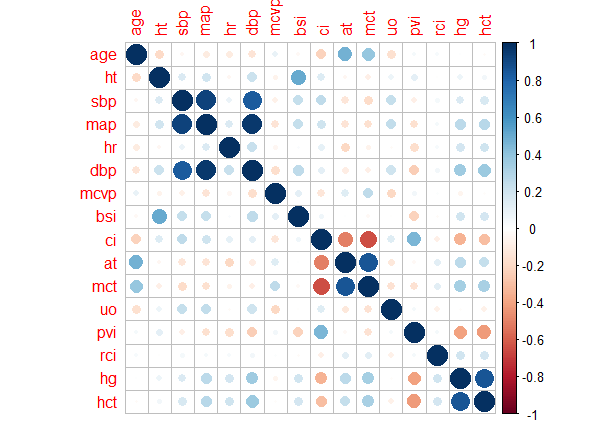
\includegraphics{cor.png}
\end{figure}

\begin{table}[ht]
\centering
\label{confuse}
\caption{Confusion Matrix}
\begin{tabular}{rrr}
  \hline
 & actual survive & actual death \\ 
  \hline
predicted survive &  49 &  11 \\ 
  predicted death &  20 &  32 \\ 
   \hline
\end{tabular}
\end{table}
\newpage
\noindent \Large{{\bf Appendix B: R Code}}
\lstinputlisting[language=R, caption =Survival Rates]{final.R}
\end{document}
